%# -*- coding: utf-8-unix -*-

\chapter{结合隐性特征的机票推荐算法}
\label{chap:latent}
我们在前几章中介绍了建立特征分布模型表达用户对机票的偏好。为用户建模的过程分为两步,首先从机票数据字段中抽取能反映机票主要内容的显性特征,再根据用户在每个特征内容上的选择分布进行用户建模。本章,我们结合机票的隐性特征建立用户偏好模型,并进行个性化机票推荐。

\section{用户出行性质对机票推荐准确率的影响}

我们将第三章中提出的用户特征分布模型进行上线部署并进行了一段时间的A/B测试对照实验。实验将用户随机分流,一部分用户(实验组)看到的候选机票列表是经过个性化推荐过后的搜索结果展示页。对于航线冷启动用户,我们在线上生产环境中采取了特征打分的原则并提供多样性推荐;其他用户(对照组)看到的是原版展示页。实验的主要观测指标是用户转化率,即订购机票的用户占浏览过机票用户总数的比例。A/B测试证实,实验组比对照组的转化率有所提升,但在周末和节假日时,实验组的转化率有所下降。我们通过分析发现,主要有两方面的原因。

\begin{figure}
 \centering
 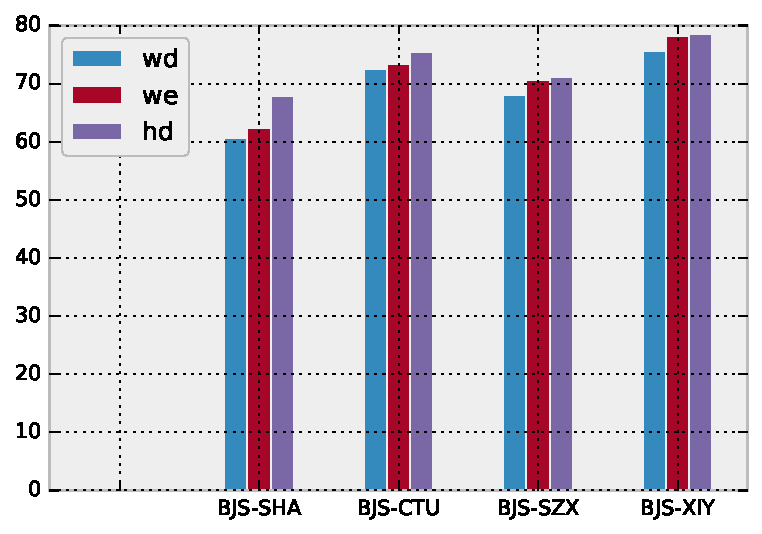
\includegraphics[width=0.6\linewidth]{04/1_inac_count.pdf}
 \bicaption[fig:inac_per]{冷启动用户占比}{不同起飞日期冷启动用户占比}{Fig}{Percentage of Inactive Users at Different Takeoff Date}
\end{figure}

图\ref{fig:inac_per}展示了在不同起飞日期航线冷启动用户占比。我们将时间分为工作日(wd)、周末(we)和节假日(hd)。可以看到,不同航线上的冷启动用户比例总体有差距。北京-上海和北京-深圳的航线冷启动用户数量处于较低比例;北京-成都和北京-西安的航线冷启动用户数量处于较高比例。对每条航线而言,工作日的航线冷启动用户占比最低;周末和节假日的航线冷启动用户占比都较高,并且比例很接近。其中以北京-上海航线的工作日和节假日的冷启动用户比例差异最大。可以发现,非活跃用户比例差异的是第一个原因。在周末和节假日,航线非活跃用户比例增加,导致推荐效果的差异。第二个原因与用户行为的改变相关。我们主要关注用户的出行性质。

用户的出行性质多种多样,如出差、参会、探亲、旅游等。总体来说可以分为商务性质和个人性质。对于出行性质是商务的乘客由于其行程安排及工作单位的差旅政策等因素,可能会更多地关注起飞时间、航空公司等特征,而对价格,舱位等特征关注较少;对于出行性质是个人的乘客,则更关注价格、退改签政策等特征。即使对于同一位用户,如果其出行性质不同,那么在购买机票时的关注点也会不同,从而产生用户行为的改变。用户的出行性质是一个无标签分类问题,它不能直接体现在订单数据中。因而我们无法对这个问题进行实验验证。但是我们可以通过直接对比推荐准确率,分析用户的行为是否产生改变。




以显性特征进行统计与分析所建立的模型在一定程度上可以很好地概括用户的习惯偏好,也具有较强的解释性。



\section{问题建模及目标函数优化}

\begin{equation}
	V(u,i) = \phi_u^T * \theta_i
\end{equation}

\begin{equation}
	\phi_u = W_u * K_u
\end{equation}

\begin{equation}
	\theta_i = M_i * F_i
\end{equation}




\begin{eqnarray}
    P(i,j) & = & P(V(u,i) > V(u,j)) \nonumber \\
	 & = &\frac{1}{1+e^{-(V(u,i) - V(u,j))}}
\end{eqnarray}

\begin{equation}
	W_u = W_u + \eta(\frac{\partial \log P(i,j)}{W_u} - \lambda*W_u)
\end{equation}

\begin{equation}
	M_i = M_i + \eta(\frac{\partial \log P(i,j)}{M_i} - \lambda*M_i)
\end{equation}

\begin{equation}
  \arg\min_{W,M} : - \log P(i,j) + \frac{\lambda}{2} * (\sum_{i,j \in W}W_{i,j}^2 + \sum_{i,j \in M}M_{i,j}^2)
\end{equation}

\begin{equation}
	R(I) =  R(P_u^T * F_I) + R(\phi_u^T * \theta_I)
\end{equation}

\section{结合隐性特征的机票个性化推荐}

\section{实验结果分析}